\chapter{Developed approach}
\label{chapter:approach}

\section{Overview}
\label{section:overview}

The auditor is a Python package (\texttt{ccauditor}, $\approx$4\,000 lines) organised as a pipeline of stages that
exchange typed data contracts (Pydantic models \texttt{Clause}, \texttt{Requirement}, \texttt{Evidence},
\texttt{Verdict}, \texttt{RiskAssessment}, \texttt{AuditReport}). The same pipeline is exposed through a CLI
(\texttt{ccauditor audit|policies|diff-policy|ci|review}), a FastAPI REST service and a Next.js web dashboard.
Figure~\ref{fig:agents} shows the agents and what each one is allowed to see and produce. Three evaluation modes share the
pipeline: \emph{deterministic} (rules only, no LLM call), \emph{llm} (the judge evaluates every applicable requirement)
and \emph{hybrid} (rules first, LLM only where needed).

\begin{figure}[htbp]
\centering
\resizebox{\linewidth}{!}{%
\begin{tikzpicture}[font=\sffamily\footnotesize,
  ag/.style={draw, rounded corners=3pt, fill=#1, align=center, text width=2.8cm, minimum height=1.25cm},
  ag/.default=violet!10,
  det/.style={draw, rounded corners=3pt, fill=green!10, align=center, text width=2.8cm, minimum height=1.25cm},
  arr/.style={-{Stealth[length=2mm]}, thick}, lab/.style={font=\sffamily\scriptsize, text=black!60, align=center}]
  \node[ag=gray!12, text width=13.6cm, minimum height=0.8cm] (orch) at (5.4,2.6)
     {\textbf{Orchestrator} (\texttt{pipeline.run\_audit}): plans the run, routes deterministic $\leftrightarrow$ LLM,
      aggregates, enforces the human gate, records timings / calls / tokens / cost};
  \node[ag] (pa) at (0,0) {\textbf{PolicyAnalyst}\\clauses $\to$ requirements\\(only if no curated YAML)};
  \node[ag] (rc) at (3.6,0) {\textbf{RiskClassifier}\\Art.~5 / Annex III /\\Art.~50 tier};
  \node[det] (re) at (7.2,0) {\textbf{Rule engine}\\pattern, file\_exists,\\yaml\_path, rego};
  \node[det] (sc) at (10.8,0) {\textbf{EvidenceScout}\\BM25 multi-query,\\no LLM};
  \node[ag] (jd) at (10.8,-2.4) {\textbf{ComplianceJudge}\\status, confidence,\\cited ids, gaps};
  \node[ag=red!8] (vf) at (7.2,-2.4) {\textbf{Verifier}\\citation existence\\(+ optional LLM support check)};
  \node[ag=yellow!20] (hl) at (3.6,-2.4) {\textbf{Human gate}\\conflicts, confidence\\$<\beta$ $\to$ review queue};
  \node[ag] (rm) at (0,-2.4) {\textbf{Remediator /}\\\textbf{ArtifactGenerator}\\fixes, draft docs};
  \foreach \n in {pa,rc,re,sc} \draw[arr, black!50] (orch.south -| \n) -- (\n);
  \draw[arr] (re) -- node[lab, above=4pt]{hint} (sc);
  \draw[arr] (sc) -- node[lab, right]{$\le$14 items,\\$\le$12k chars} (jd);
  \draw[arr] (jd) -- (vf);
  \draw[arr] (vf) -- (hl);
  \draw[arr] (hl) -- (rm);
  \node[lab] at (5.4,-3.75) {violet: LLM agent (Claude, headless, no tools)\quad green: deterministic\quad red/yellow: safeguards};
\end{tikzpicture}}
\caption{Agents of the auditor. Every LLM agent is a single structured (JSON-schema) call without tool access; the
orchestrator is ordinary code, so the control flow is fixed and auditable.}
\label{fig:agents}
\end{figure}

\section{Policy ingestion and decomposition}
\label{section:policies}

Policies are stored as markdown with a YAML front matter (\texttt{id}, \texttt{version}, \texttt{source}); headings
``\texttt{\#\# Art.~12 | Record-keeping}'' and ``\texttt{\#\#\# 1}'' are parsed into clauses with stable, citable ids
(\texttt{eu-ai-act/Art.12}, \texttt{eu-ai-act/Art.12(1)}) and parent links. Requirements are \emph{curated} in YAML
(statement, clause ids, category, applicable risk tiers, severity, retrieval queries, judge guidance and deterministic
checks). When no curated file exists for a policy, the \textbf{PolicyAnalyst} agent decomposes the clauses in batches,
with the instruction to emit only atomic, repository-testable requirements, to use only the given clause ids and to skip
definitional or authority-facing clauses. Table~\ref{tab:corpus} summarises the bundled corpus. A \textbf{policy
evolution} module diffs two versions of a policy at clause level (added / removed / modified, with parent--child
propagation) and lists the requirements and existing reports impacted by the change.

\begin{table}[htbp]
\caption{Policy corpus and curated requirements.}
\label{tab:corpus}
\centering\small
\begin{tabular}{@{}lrrrrl@{}}
\toprule
\textbf{Policy} & \textbf{Clauses} & \textbf{Req.} & \textbf{with checks} & \textbf{checks} & \textbf{check types} \\
\midrule
EU AI Act (selected provisions) & 108 & 23 & 22 & 25 & 19 pattern, 6 file\_exists \\
GDPR (selected articles) & 32 & 11 & 10 & 12 & 9 pattern, 3 file\_exists \\
ACME RAI policy (fictional, v1) & 30 & 11 & 10 & 12 & 11 pattern, 1 file\_exists \\
\midrule
\textbf{Total} & 170 & 45 & 42 & 49 & \\
\bottomrule
\end{tabular}
\end{table}

\section{Evidence collection and retrieval}
\label{section:evidence}

The collector walks the repository (skipping binaries, vendored and build directories), classifies each file into one of
six evidence kinds (code, config, IaC, doc, model card, log) and splits it into overlapping windows of 40 lines (overlap
10; files of at most 50 lines are a single chunk). Each chunk receives a stable id (hash of path and line span) and the
set of \emph{signals} raised by 16 lightweight regex detectors (logging call, AI disclosure, human override, retention
configuration, PII field, model call, consent, encryption, access control, rate limit, data documentation,
bias/fairness, accuracy metrics, risk management, monitoring, anonymisation).

Retrieval uses BM25~\cite{robertson2009bm25} over path + snippet with a code-aware tokenizer (camelCase and snake\_case
are split, the joined form is kept), boosted by $1.5\times$ when a query term matches a chunk signal. The
\textbf{EvidenceScout} builds several queries per requirement (curated queries, keywords of title + statement, one
category-specific expansion), merges the hits with a reciprocal-rank bonus, \emph{pins} the evidence already cited by the
rule engine first, and caps the result at 14 items and 12\,000 characters (1\,500 per snippet). No embedding model is
needed and the scout makes no LLM call.

\section{Risk-tier classification}
\label{section:risk}

Applicability depends on the AI Act tier. A deterministic pre-classifier matches regex triggers for prohibited practices
(Art.~5: social scoring, manipulation, workplace emotion recognition, untargeted facial scraping, predictive policing,
real-time remote biometric identification), Annex~III high-risk areas (biometrics, critical infrastructure, education,
employment, credit scoring, \dots) and Art.~50 transparency cases (chatbots, generative content, deep fakes) mostly in
documentation. Negated mentions are ignored (``the system does not interact with people as a chatbot'') and matches
are weighted by where they occur: a self-description in the README or model card counts 2.0, other documents 1.0 and
code 0.5, capped at 1.0 for code alone. A tier needs a score of at least 2. The classifier returns the most severe tier
together with the triggering evidence. In LLM modes the \textbf{RiskClassifier}
agent receives this result as a hint plus retrieved descriptions of the intended purpose, and returns tier, triggers and
cited evidence. Requirements whose $A_r$ excludes the tier get \stat{na} deterministically (Eq.~\ref{eq:applic}); the
judge is not allowed to output \stat{na}.

\section{Deterministic rule engine}
\label{section:rules}

Each check returns \emph{pass}, \emph{fail} or \emph{unknown}: \texttt{pattern} (a regex must be present / absent in files
selected by glob or evidence kind), \texttt{file\_exists}, \texttt{yaml\_path} (a key exists or equals a value in
YAML/JSON) and \texttt{rego} (evaluated with OPA~\cite{opa} if installed, otherwise unknown). Results are aggregated per
requirement: all resolved checks pass $\Rightarrow$ \stat{c}; none pass $\Rightarrow$ \stat{nc}; mixed $\Rightarrow$
\stat{p}; no resolved check $\Rightarrow$ \stat{nr}. The engine cites the matching chunks and lists the failed
checks as gaps.

\paragraph{Comment awareness.} Pattern checks run on a copy of each file in which comments, docstrings and
TODO/FIXME/TBD lines are blanked out; line numbers are preserved. Python is handled with \texttt{tokenize}; C-like,
hash, HCL, SQL and markup comments are handled by a string-aware scanner. Commented-out code and TODOs are treated as
non-evidence. Explanatory prose comments count only as a weak claim. Switched-off flags such as
\texttt{override\_allowed = False} do not satisfy a ``present'' check.

\paragraph{Graded confidence.} Each check outcome carries a strength. It depends on the number of matching lines and
files, on the evidence kind (a technical requirement satisfied only by documentation is a \emph{claim}, 0.55) and on
the check type (regex miss 0.6, ``absent'' pass 0.6, file exists 0.7, \dots). The verdict's confidence is the mean
strength of its decisive checks, plus $0.05$ when at least two independent checks agree, capped at $0.95$. \stat{p} and
\stat{nr} keep defaults of $0.5$ and $0.2$. The baseline (v0) instead used fixed priors: $0.9$ for \stat{c} and $0.8$
for \stat{nc}.

\section{LLM judge}
\label{section:judge}

The \textbf{ComplianceJudge} receives one requirement (statement, guidance, the text of its source clauses), the scout's
evidence rendered with short aliases (\texttt{[E1]}, \texttt{[E2]}, \dots, which are far less error-prone than hash ids),
and, in hybrid mode, the rule-engine verdict explicitly labelled as a hint that ``can be wrong (regexes are shallow)''.
The system prompt fixes the contract:
\begin{itemize}[leftmargin=*]
  \item decide only from the excerpts and cite only the given ids;
  \item absence of evidence is not compliance;
  \item use \stat{nr} only for genuinely ambiguous evidence;
  \item report a calibrated confidence (below 0.6 when unsure);
  \item list concrete gaps and an actionable remediation.
\end{itemize}
It also states the labelling rubric:
\begin{itemize}[leftmargin=*]
  \item the statement is the test, so the judge must not demand more than it says;
  \item an excerpt truncated at a chunk boundary is not a gap;
  \item claims and TODOs are not evidence;
  \item \stat{c}, \stat{p} and \stat{nc} have explicit meanings, and a missing artefact is \stat{nc}.
\end{itemize} The answer must follow a JSON schema
(\texttt{status, confidence, rationale, evidence\_ids, gaps, remediation}); aliases are mapped back to evidence ids, and
unknown ids are kept verbatim so that the Verifier can remove them.

\section{Hybrid orchestration}
\label{section:hybrid}

Algorithm~\ref{alg:hybrid} gives the orchestration. Two thresholds control the trade-off between cost and quality.
\begin{itemize}[leftmargin=*]
  \item The \emph{routing threshold} $\tau=0.675$ applies to the graded rule confidence. It was chosen by
        leave-one-app-out cross-validation (Section~\ref{section:results}) and sends about 60\% of the applicable items
        to the judge. Every \stat{p} or \stat{nr} rule verdict, and every requirement that has judge guidance but no
        checks, is always routed.
  \item The \emph{human-review threshold} is $\beta=0.6$.
\end{itemize}
The \textsc{Combine} step arbitrates transparently. On a hard disagreement (\stat{c} vs.\ \stat{nc}), the side that is
at least $\delta=0.15$ more confident wins; its confidence is lowered by $0.1$ and both rationales are recorded.
Otherwise the item becomes \stat{nr} for a reviewer. When the rules and the judge agree, the confidence rises by
$0.05$.

\algsetup{indent=1.5em, linenosize=\footnotesize}
\begin{algorithm}[htbp]
\caption{Hybrid audit orchestration (\texttt{pipeline.run\_audit}, mode = hybrid)}
\label{alg:hybrid}
\begin{algorithmic}[1]
\REQUIRE repository $D$, policy ids, LLM backend $B$, thresholds $\tau=0.675$, $\beta=0.6$, margin $\delta=0.15$
\ENSURE audit report with verdicts $V$, scorecard, statistics
\STATE $\Req \leftarrow$ curated requirements, or \textsc{PolicyAnalyst}$_B$(clauses) if none
\STATE $\Ev \leftarrow \varphi(D)$; build BM25 index over $\Ev$
\STATE $t \leftarrow$ \textsc{RiskClassifier}$_B$($\Ev$, hint = \textsc{HeuristicTier}($\Ev$))
\STATE $J \leftarrow \emptyset$ \COMMENT{requirements routed to the LLM judge}
\FORALL{$r \in \Req$}
  \IF{$t \notin A_r$}
    \STATE $V[r] \leftarrow (\stat{na}, \text{conf}(t), \emptyset)$; \textbf{continue}
  \ENDIF
  \STATE $d_r \leftarrow$ \textsc{Verify}(\textsc{RuleEngine}($r, D, \Ev$), ids$(\Ev)$, requireEvidence = false)
  \IF{$d_r.\text{status}\in\{\stat{p},\stat{nr}\}$ \OR $d_r.\text{conf} < \tau$ \OR ($K_r=\emptyset$ \AND $g_r \neq \varepsilon$)}
    \STATE $J \leftarrow J \cup \{r\}$
  \ELSE
    \STATE $V[r] \leftarrow d_r$ \COMMENT{confident rule verdict, no LLM call}
  \ENDIF
\ENDFOR
\FORALL{$r \in J$ \textbf{in parallel} (bounded by the backend concurrency)}
  \STATE $\Ev_r \leftarrow$ \textsc{EvidenceScout}($r$, pinned $=d_r$.ids) \COMMENT{BM25, $\le 14$ items}
  \STATE $\ell_r \leftarrow$ \textsc{ComplianceJudge}$_B$($r$, $\Ev_r$, hint $=d_r$)
  \STATE $\ell_r \leftarrow$ \textsc{Verifier}($r$, $\ell_r$, $\Ev_r \cup d_r$.ids) \COMMENT{Algorithm~\ref{alg:verifier}}
  \IF{$\{d_r.\text{status}, \ell_r.\text{status}\} = \{\stat{c},\stat{nc}\}$}
    \IF{$|\ell_r.\text{conf} - d_r.\text{conf}| \ge \delta$}
      \STATE $v \leftarrow$ more confident side, conf $- 0.1$, keep both rationales
    \ELSE
      \STATE $v \leftarrow (\stat{nr}, \min(0.5, d_r.\text{conf}, \ell_r.\text{conf}))$, keep both rationales
    \ENDIF
  \ELSIF{$d_r.\text{status} = \ell_r.\text{status}$}
    \STATE $v \leftarrow \ell_r$ with conf $\leftarrow \min(1, \max(d_r.\text{conf}, \ell_r.\text{conf}) + 0.05)$
  \ELSE
    \STATE $v \leftarrow \ell_r$ \COMMENT{e.g.\ rule \stat{p}, judge \stat{c}}
  \ENDIF
  \STATE $v \leftarrow$ \textsc{Verify}($v$, $\Ev_r \cup d_r$.ids)
  \IF{$v.\text{status}\notin\{\stat{nr},\stat{na}\}$ \AND $v.\text{conf} < \beta$}
    \STATE $v.\text{status} \leftarrow \stat{nr}$ \COMMENT{human-in-the-loop gate}
  \ENDIF
  \STATE $V[r] \leftarrow v$
\ENDFOR
\STATE scorecard $\leftarrow$ \textsc{Score}($\Req, V$); record timings, calls, tokens, cost, cache hits
\RETURN report($t$, $V$, cited evidence, scorecard, statistics)
\end{algorithmic}
\end{algorithm}

\section{Verifier: anti-hallucination contract}
\label{section:verifier}

The Verifier (Algorithm~\ref{alg:verifier}) enforces Eqs.~(\ref{eq:ground})--(\ref{eq:support}). Its deterministic pass
runs on \emph{every} verdict, including rule-engine ones: citations that do not belong to the evidence actually shown to
the evaluator are removed and the confidence is multiplied by $0.8$; a positive verdict (\stat{c} or \stat{p}) without
any remaining valid citation is downgraded to \stat{nr} with confidence at most $0.4$ (``no hallucinated compliance'').
An optional LLM pass, in the spirit of attribution checking~\cite{rashkin2023ais,min2023factscore}, shows a second,
sceptical model only the cited excerpts and asks whether they support the claim; unsupported claims become \stat{nr}
while the citations stay visible to the reviewer.

\begin{algorithm}[htbp]
\caption{Verifier (\texttt{agents/verifier.py})}
\label{alg:verifier}
\begin{algorithmic}[1]
\REQUIRE requirement $r$, verdict $v=(y,\pi,\hat E)$, evidence set provided to the evaluator $\Ev_r$, flag \textit{useLLM}
\ENSURE verified verdict
\STATE \textsc{Check}:
\STATE \quad $\hat E_{\text{bad}} \leftarrow \hat E \setminus \Ev_r$; \quad $\hat E \leftarrow \hat E \cap \Ev_r$
\IF{$\hat E_{\text{bad}} \neq \emptyset$}
  \STATE $\pi \leftarrow 0.8\,\pi$; append ``removed $|\hat E_{\text{bad}}|$ citation(s)'' to the rationale
\ENDIF
\IF{\textit{requireEvidence} \AND $y \in \{\stat{c}, \stat{p}\}$ \AND $\hat E = \emptyset$}
  \STATE $y \leftarrow \stat{nr}$; $\pi \leftarrow \min(\pi, 0.4)$ \COMMENT{no compliance without evidence}
\ENDIF
\STATE mark $v$ as verified
\IF{\textit{useLLM} \AND $y \in \{\stat{c}, \stat{p}\}$}
  \STATE $(s, U) \leftarrow$ LLM(``do excerpts $\hat E$ support status $y$ for statement $s_r$?'')
  \STATE $\hat E \leftarrow \hat E \setminus U$
  \IF{$s = \text{false}$ \OR $\hat E = \emptyset$}
    \STATE $y \leftarrow \stat{nr}$; $\pi \leftarrow \min(\pi, 0.5)$; keep original citations for the reviewer
  \ENDIF
\ENDIF
\RETURN $(y, \pi, \hat E)$
\end{algorithmic}
\end{algorithm}

\section{Human review, scoring and reporting}
\label{section:report}

Every verdict carries status, confidence, method (deterministic / llm / hybrid / human), a \emph{verified} flag,
rationale, gaps, remediation and the cited evidence with path and line span. Reviewers resolve \stat{nr} items (or
contest any other verdict) by submitting a decision with their name and a justification; the override is recorded in the
rationale and in the report history, the method becomes \texttt{human} and the scorecard is recomputed. Category scores
are $(\#\stat{c} + 0.5\,\#\stat{p}) / \#\text{applicable} \times 100$; the overall score uses the same credit weighted by
severity (critical 4, high 3, medium 2, low 1). Reports are rendered as JSON, Markdown and SARIF~\cite{sarif2020} (so
that gaps appear as code-scanning alerts on the cited lines), and an \texttt{explain} function prints the full
justification of a single verdict. The \textbf{ArtifactGenerator} drafts missing artefacts (technical documentation,
risk assessment, transparency notice, model card~\cite{mitchell2019modelcards}) from the findings, with explicit
\texttt{[TODO]} placeholders instead of invented facts.

\section{LLM backend, caching and CI}
\label{section:backend}

The LLM is Claude, called through the \textbf{Claude Code CLI in headless mode}~\cite{claudecode}
(\texttt{claude -p --output-format json --json-schema ...}) with the developer's subscription, so no API key is stored.
Each call runs with tools, MCP servers, slash commands, settings and session persistence disabled, in an empty temporary
working directory: the model can read only the prompt. Responses are parsed (with a fallback that extracts the first
balanced JSON object), validated against the schema and retried up to twice with the validation errors appended. A
content-addressed \textbf{disk cache} (SHA-256 of model, system prompt, prompt and schema) makes re-audits of unchanged
code free and deterministic; the backend records calls, cache hits, failures, input/output tokens, the equivalent USD
cost reported by the CLI and latency. A semaphore bounds the concurrency (default 4). A \texttt{FakeBackend} makes the
whole pipeline testable offline. In CI, \texttt{ccauditor ci} audits the current tree, compares it with a baseline report
(per-requirement status rank $\stat{nc} < \stat{nr} < \stat{p} < \stat{c}$) and fails the build on regressions at or above
a chosen severity.

\section{Web dashboard}
\label{section:web}

The Next.js dashboard (over the REST API: \texttt{/policies}, \texttt{/audit}, \texttt{/reports/compare},
\texttt{/reports/render}, \texttt{/reports/review}, \texttt{/policies/diff}) lets a user browse policies and clauses, launch
an audit (mode, policies, model), and inspect a report in four tabs: \emph{overview} (score gauge, per-category charts, risk
tier and triggers), \emph{requirements} (filterable table; a side sheet shows the statement, source clauses, rationale,
cited code snippets, gaps and remediation), \emph{review} (the human-in-the-loop queue with a decision form) and
\emph{traceability} (clause $\to$ requirement $\to$ evidence links). Figure~\ref{fig:dashboard} shows the report of
\texttt{hireright-screening} in hybrid mode.

\begin{figure}[htbp]
\centering
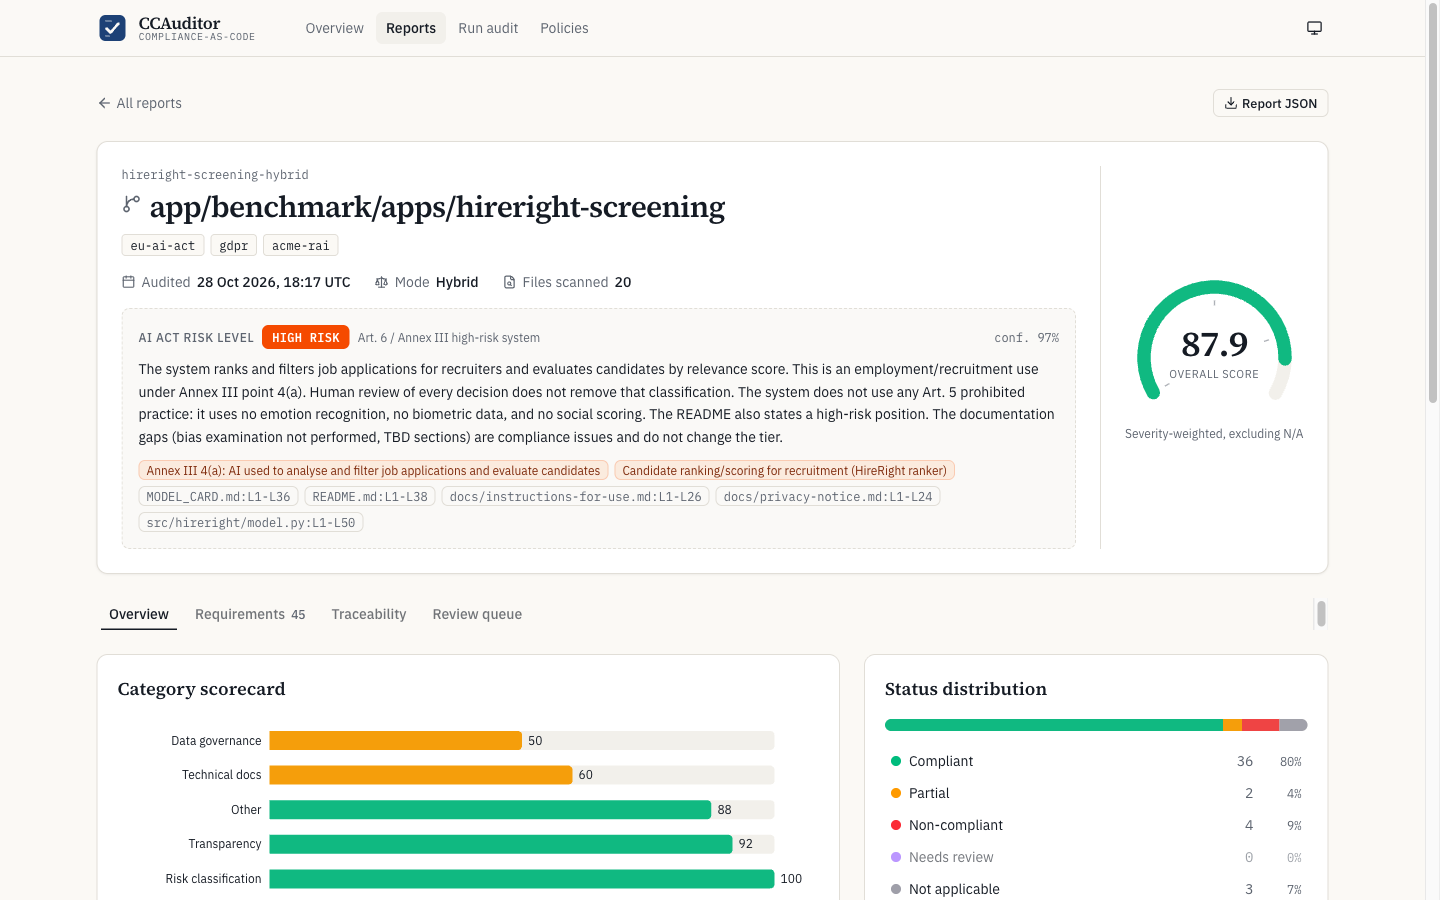
\includegraphics[width=0.6\linewidth]{figures/dashboard_overview.png}\hfill
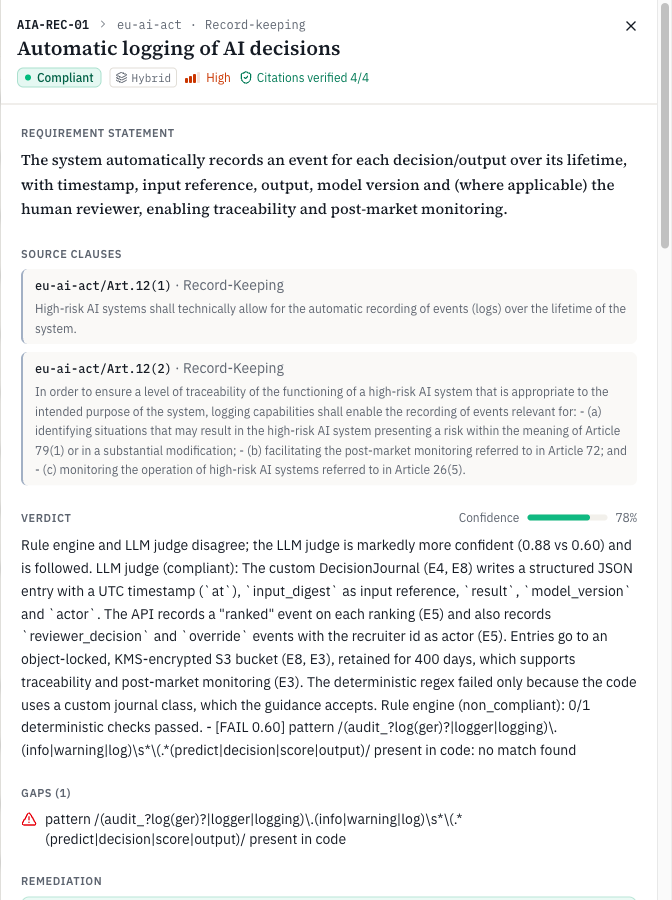
\includegraphics[width=0.38\linewidth]{figures/dashboard_requirement.png}
\caption{Web dashboard, \texttt{hireright-screening} audited in hybrid mode. Left: the overview, with the risk tier, its
triggers and cited files, the severity-weighted score and the category scorecard. Right: the requirement drawer for
\texttt{AIA-REC-01}, showing the statement, the source clauses, the verdict with its confidence and the arbitration
rationale (rule engine vs.\ LLM judge), verified citations and gaps. Further down the drawer are the cited code and
the human-review form.}
\label{fig:dashboard}
\end{figure}

\section{Worked example}
\label{section:example}

Consider requirement \texttt{AIA-REC-01} on \texttt{hireright-screening}, a high-risk CV-ranking service (Annex~III
4(a)). The requirement derives from Art.~12(1)--(2): every decision must be logged automatically with a timestamp, an
input reference, the output and the model version. The ground truth is \stat{c}, because every ranking is recorded by a
custom \texttt{DecisionJournal.record(...)} on S3 Object Lock, and no \texttt{logger} call is used.
\begin{enumerate}[leftmargin=*]
  \item The tier is \emph{high}, triggered by the recruitment description in the README and the model card, so the
        requirement applies.
  \item The rule check is a regex for a \texttt{logger} or \texttt{audit\_log} call in code that mentions a prediction,
        decision, score or output. It does not match, so the rule engine says \stat{nc}.
  \item \textbf{v0:} the fixed prior gave this verdict confidence $0.8 \ge 0.75$, so hybrid mode kept the confident but
        wrong \stat{nc} without asking the LLM. The deterministic and hybrid modes were both wrong. LLM-only mode was
        right (\stat{c}, 0.82, 5 citations).
  \item \textbf{v1:} a regex miss is graded at $0.6 < \tau$, so the item is routed. The scout's queries ``journal
        record decision'' and ``audit log decision'' retrieve \texttt{journal.py}, the call sites in \texttt{api.py}
        and the retention configuration. The judge answers \stat{c} with confidence 0.88 and cites 4 excerpts. The
        judge is $0.28 \ge \delta$ more confident than the rules, so it wins the arbitration. The final verdict is
        \stat{c} with confidence 0.78, and both rationales stay visible (Figure~\ref{fig:dashboard}, right).
\end{enumerate}
The example shows the central trade-off quantified in Chapter~\ref{chapter:experiments}. Confident rules save LLM calls
but propagate their false negatives. Graded confidence makes a ``regex miss'' weak enough to be checked, while strong
rule evidence still saves the call.
